\documentclass[border=4pt]{standalone}

% --- packages (mirror these in user.meta.json "requires") ---
\usepackage{tikz}

% --- palette (canonical source: skills/color-palettes/skill.md; light variant) ---
\definecolor{otblue}{HTML}{0072B2}
\definecolor{otorange}{HTML}{E69F00}
\definecolor{otteal}{HTML}{009E73}
\definecolor{otpurple}{HTML}{CC79A7}
\definecolor{otgray}{HTML}{5A5A5A}

\begin{document}
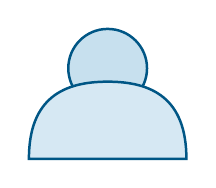
\begin{tikzpicture}[line width=0.9pt]
  % head
  \filldraw[draw=otblue!75!black, fill=otblue!22] (0,1.15) circle[radius=0.5];
  % shoulders
  \filldraw[draw=otblue!75!black, fill=otblue!16]
    (-1.0,0) .. controls (-1.0,0.78) and (-0.55,0.98) .. (0,0.98)
    .. controls (0.55,0.98) and (1.0,0.78) .. (1.0,0) -- cycle;
\end{tikzpicture}
\end{document}
